\setmainfont{Noto Serif}
\setsansfont{Noto Sans}
\setmonofont{Noto Sans Mono}
\setstretch{1.35}
\hyphenation{ма-те-ма-ти-ка вос-ста-нав-ли-вать}
\input{insbox}

\section{Электронное строение многоатомных молекул}
1К. Определите поляризацию самой длинноволновой линии поглощения линейного катион-радикала $\text{BeH}_2^{+\boldsymbol{\cdot}}$. Потенциал ионизации $1s$ электрона водорода равен 13,6 эВ, $2s$ электрона атома бериллия 9,3 эВ. Разница между $2s$ и $2p$ подуровнями в атоме бериллия равна 3,4 эВ.
\par
%\vspace{\parskip}
%\InsertBoxR{0}{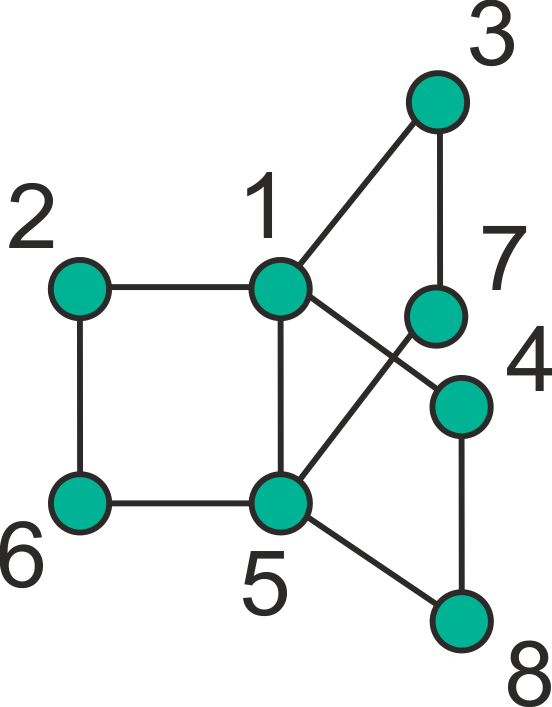
\includegraphics[width=10mm,height=10mm,keepaspectratio]{images/Fig_1_7_1.png}}[0]
\begin{wrapfigure}{r}{20mm} %this figure will be at the right
    \centering
    \vspace{-5.6ex}
     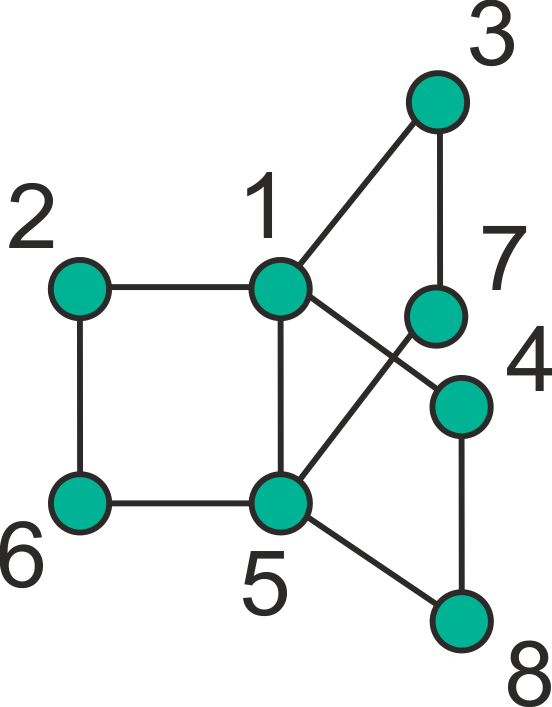
\includegraphics[width=14mm]{images/Fig_1_7_1.png}
    \vspace{-6mm}
\end{wrapfigure}
%\vspace{0.5pc}
2С. В базисе $1s$ орбиталей определите электронное строение хюккелевской системы, строение которой приведено на рисунке справа. Определите основной терм, а также количество разрешенных электрических дипольных переходов.
\par
3С. С помощью теории МО ЛКАО рассмотрите электронное строение молекулы озона, считая ее линейной. Определите основной терм.
\par
%\vspace{\parskip}
%\InsertBoxR{0}{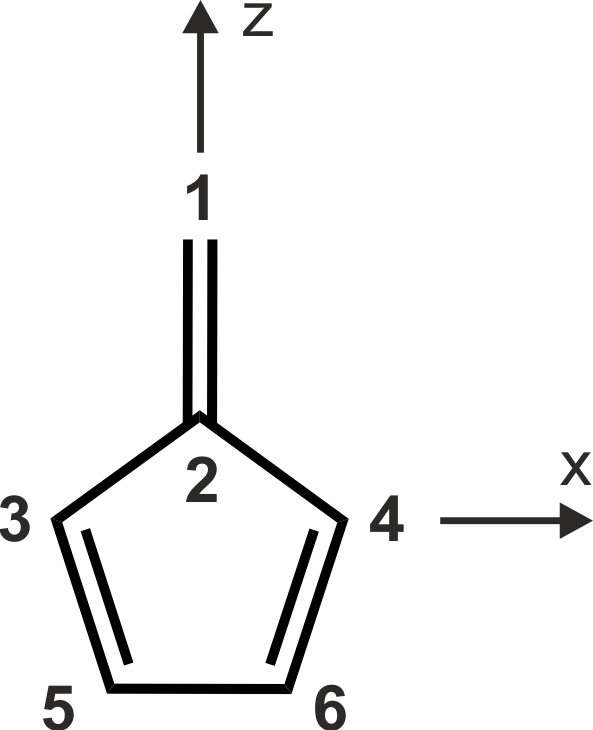
\includegraphics[width=10mm,height=10mm,keepaspectratio]{images/Fig_1_7_2.png}}[3]
\begin{wrapfigure}{r}{20mm} %this figure will be at the right
    \centering
    \vspace{-8.5mm}
    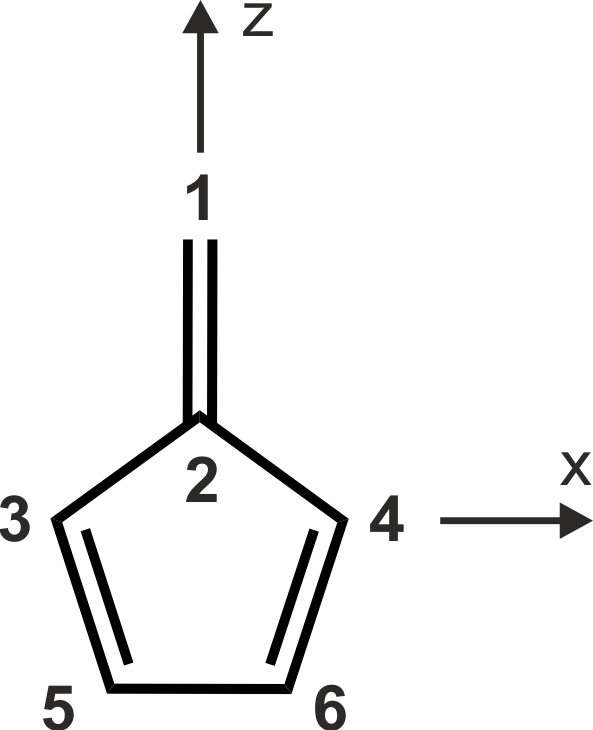
\includegraphics[width=17mm]{images/Fig_1_7_2.png}
    \vspace{-5mm}
\end{wrapfigure}
4К. Определите энергетические уровни $\pi$-системы изомера бензола – фульвена, структурная формула которого приведена на~рисунке. Чем может быть вызвано наличие большого дипольного момента у данной молекулы?
\par
5К. Используя теорию МО ЛКАО качественно определите электронное строение молекулы метана. Определите терм основного состояния нейтральной молекулы и ее катион- и анион-радикалов. Какой из указанных ионов/молекулы обладает наибольшей устойчивостью?
\par
\begin{wrapfigure}{r}{20mm} %this figure will be at the right
    \centering
    \vspace{0mm}
    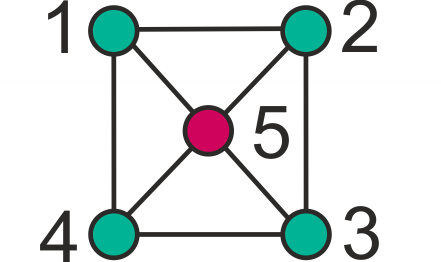
\includegraphics[width=17mm]{images/Fig_1_7_6.png}
    \vspace{-3.6mm}
\end{wrapfigure}
6С. Определите спиновую плотность хюккелевской системы, строение которой приведено на рисунке справа, в базисе $2p_z$ орбиталей. Как изменится полная электронная энергия данной системы при замене центрального атома, с кулоновским интегралом равным $\alpha$, на другой атом, с кулоновским интегралом равным $1,1\alpha$. Считайте, что резонансные интегралы при этом не изменились.
\par
7К. Постройте корреляционную диаграмму трех первых синглетных термов молекулы воды при изменении угла $\text{H}-\text{O}-\text{H}$ от 110º до 180º. Относительные энергии термов равны, соответственно, $^1A_1$, $^1B_1$, $^1A_2$: 0,0 эВ, 7,2 эВ, 8,0 эВ и $^1\Sigma _g^+$, $^1\Pi _u$, $^1\Pi _g$: 2,0 эВ, 6,4 эВ, 11,2 эВ. Каким электронным конфигурациям соответствуют указанные термы? Энергии атомных орбиталей кислорода и водорода равны: $E(2s,\text{O})$ = $-$32,4 эВ, $E(2p,\text{O})$ = $-$15,9 эВ, $E(1s,\text{H})$ = $-$13,6 эВ. При рассмотрении нелинейной молекулы воды считайте, что ось $x$ перпендикулярна плоскости молекулы.
\par
8К. Определите энергетические уровни и полную электронную энергию $\pi$-сис-темы аллильного радикала учитывая перекрывание $p_z$ орбиталей, которое задается интегралом перекрывания $S$. Считайте, что $S$ равен 0,25 для $p_z$ орбиталей соседних центров и равен 0 в ином случае. Сравните результат со~стандартным методом Хюккеля.
\par
9. Определите электронное строение ферроцена.
\par
\begin{wrapfigure}{r}{20mm} %this figure will be at the right
    \centering
    \vspace{0mm}
    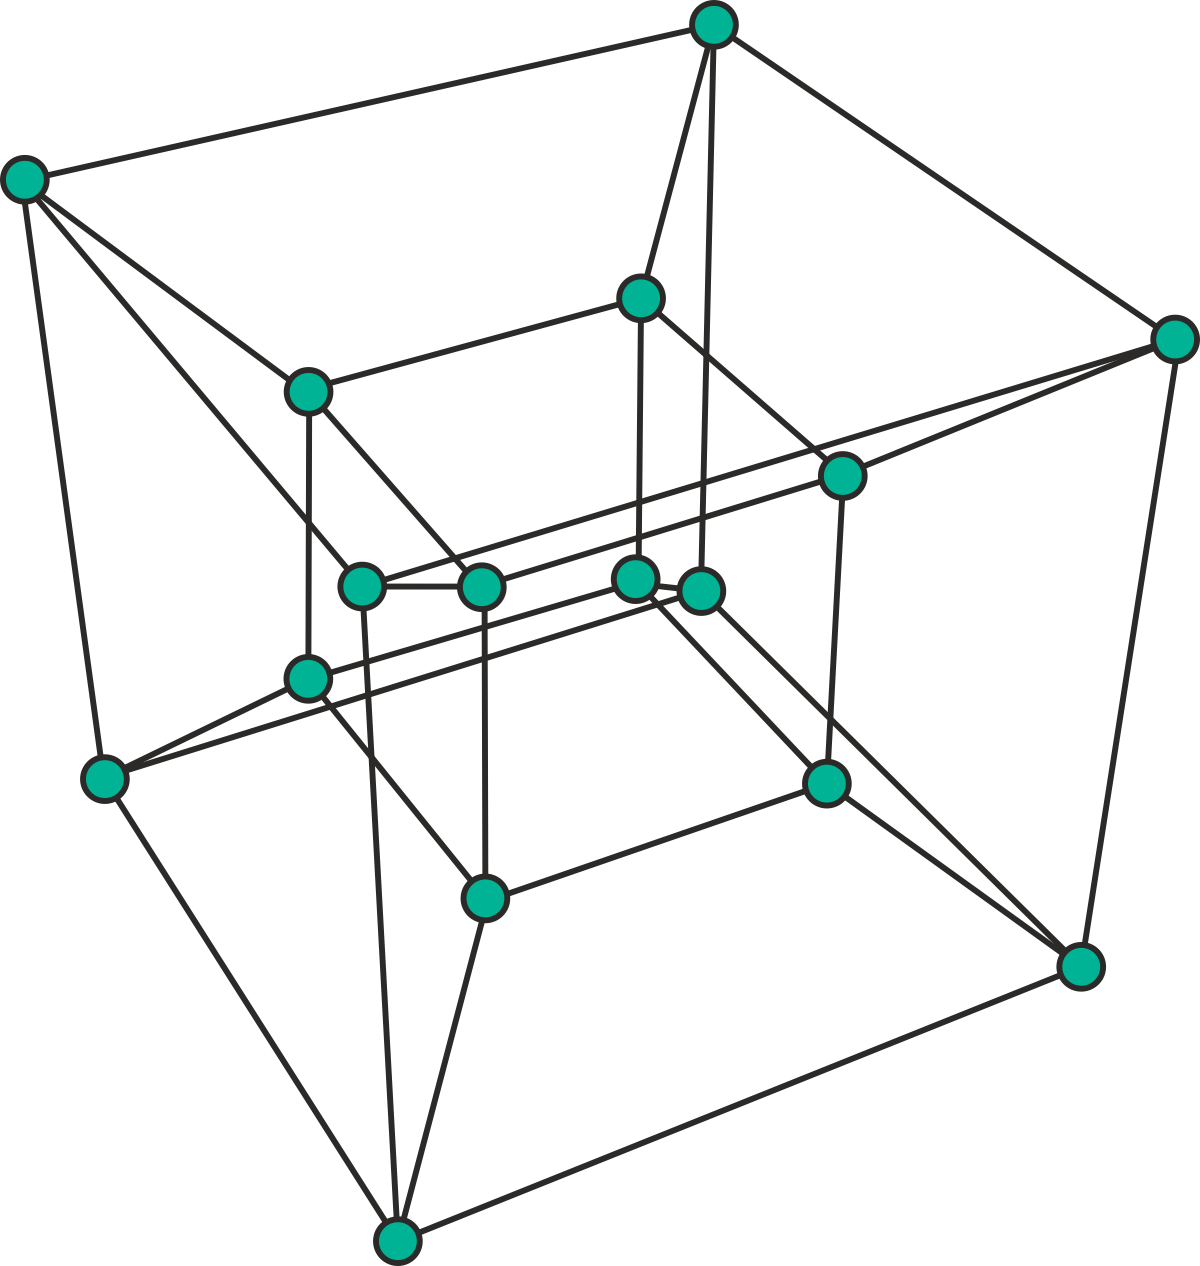
\includegraphics[width=20mm]{images/Fig_1_7_10.png}
    \vspace{-4mm}
\end{wrapfigure}
10К. В базисе $1s$ атомных орбиталей определите электронное строение (энергии и кратности вырождения всех молекулярных орбиталей) произвольной хюккелевской системы c $2^n$ центрами, где $n=0, 1, 2,\ldots$ относящейся к ряду гиперкубов: 0-куб ($n=0$, изолированный центр), 1-куб ($n$ = 1, линейная система из 2 центров), 2-куб ($n$ = 2, квадрат), 3-куб ($n$ = 3, куб), 4-куб ($n$ = 4, тессеракт) и т.д. Двухмерная проекция тессеракта приведена на рисунке справа. Определите также полную электронную энергию описанной в задаче системы для произвольного $n$. Ответ не должен содержать символ суммирования.
\par
\begin{wrapfigure}{r}{20mm} %this figure will be at the right
    \centering
    \vspace{-9mm}
    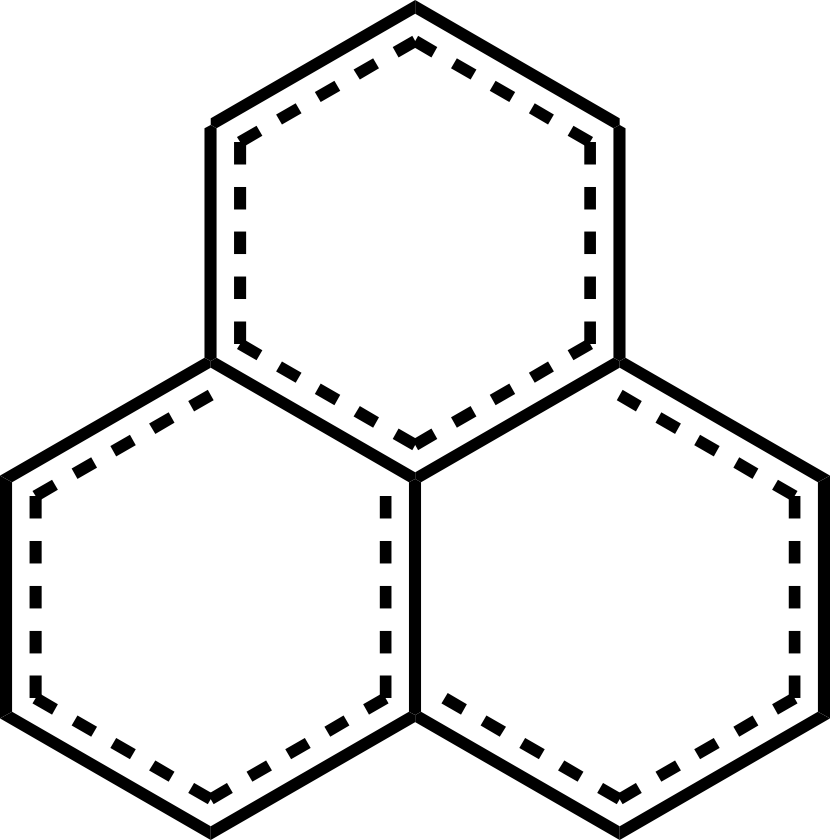
\includegraphics[width=16mm]{images/Fig_1_7_11.png}
    \vspace{-7mm}
\end{wrapfigure}
11. Определите электронное строение $\pi$-системы феналенила, структура которого приведена на рисунке. Сравните результат с теорией возмущений.
\par
12К. Определите поляризацию самой коротковолновой линии в~спектре поглощения $\pi$-системы пентадиенильного радикала.
\par
\begin{wrapfigure}{r}{30mm} %this figure will be at the right
    \centering
    \vspace{-9mm}
    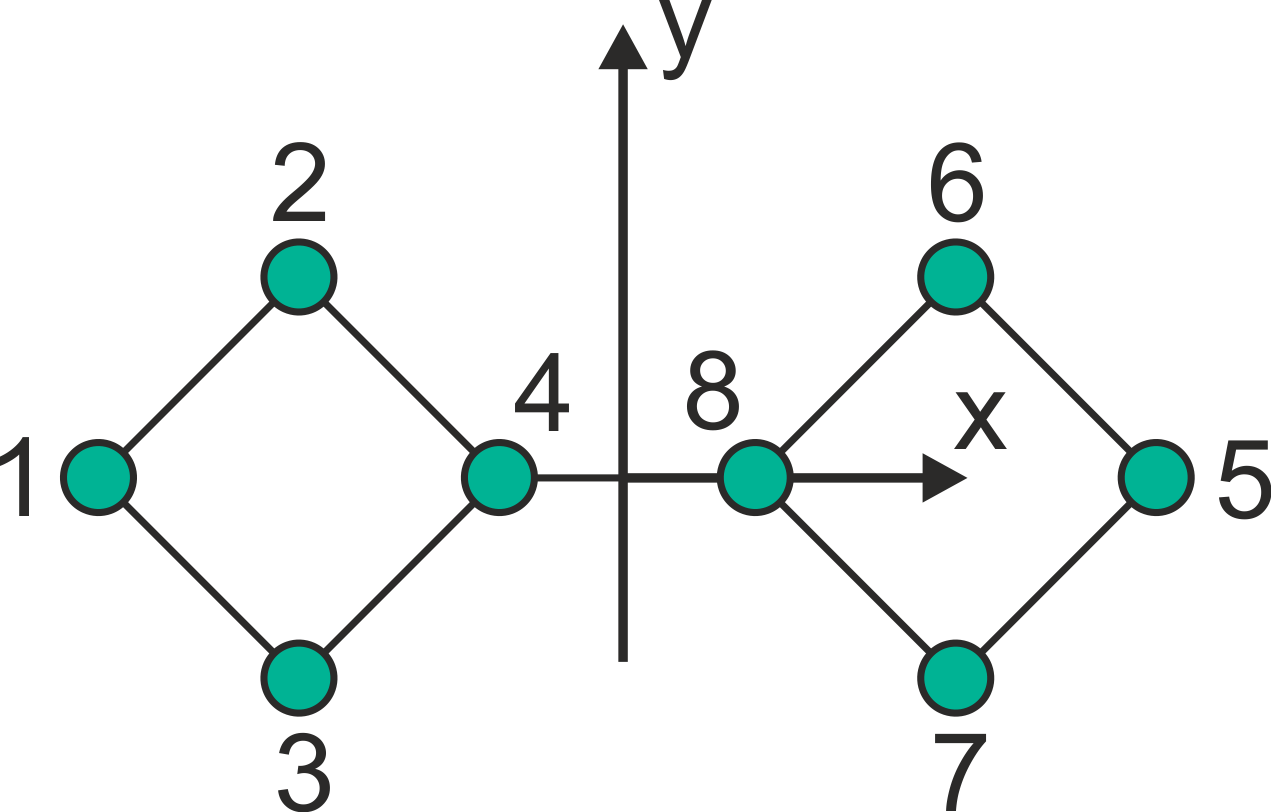
\includegraphics[width=27mm]{images/Fig_1_7_13.png}
    \vspace{-6mm}
\end{wrapfigure}
13К. Определите энергетические уровни и основной терм хюккелевской системы, изображенной на рисунке, в базисе $2p_z$ орбиталей. Все резонансные интегралы одинаковые.
\par